% !TeX root = ../main.tex
% Add the above to each chapter to make compiling the PDF easier in some editors.

\chapter{Background}\label{chapter:background}

In this chapter, we explore the current state of the field of computational humour and the needed technologies to implement the system. To be able to conduct the necessary experiment on how people react to joking robots, we require an embodied humanoid robot capable of recording video and audio data. To sustain a conversation, the robot needs a Natural-Language-based Dialogue System (in our case, the language is English). We will need a solution to store the humour-related information about users persistently. This chapter also covers our approach to the emotion recognition task for the experiment. \par

\section{What or who is Roboy?}
Roboy 3.0 is the robot build by the team of the Roboy project in February 2020. It is the third generation of Roboy’s robots. Initially, the project started as collaboration around Prof. Rolf Pfeifer at the University of Zurich in 2013~\parencite{IJCAI136900}. Currently, the project resides in Munich and Zurich.

Roboy is an Anthropomimetic Robot. Its musculoskeletal design uses elastic materials to mimic biological muscles and tendons, enhancing dexterity and adaptivity by using tendons routed along its joints and pulled by motors. Roboy 3.0 is in the top of its kind regarding the mechatronic design~\parencite{cardsflow}. However, its social interaction capabilities could be better. Thus, we will use this opportunity to conduct the research to use the results for improving Roboy’s verbal Human-Robot Interaction capabilities.
    
\section{Dialogue System}\label{section:dialogues}
To interact with robots, we use Dialogue Systems which provide knowledge extraction and processing capabilities for interaction in natural languages. A conventional Dialogue System can accept an input utterance, gauge its semantics, create a response utterance and provide an output. Most of these systems support interaction via spoken or written means, carried out directly or over social media messages. At Roboy, we developed the Ravestate framework to provide the Dialogue System functionality for our robots.

\subsection{Ravestate}

Ravestate is a framework that provides a real-time modular Dialogue System by incorporating event-based and reactive Software Engineering approaches (see Figure ). Essentially, the systems is a state machine which offers the following abstractions to implement a reactive conversation flow:

\begin{itemize}
    \item context, defined as a dictionary which keeps track of the spikes in the system.
    \item properties, defined as context variables that hold necessary values for states to functions.
    \item signals, defined as variables that can be emitted, which causes a spike in the context.
    \item states, defined as conditions and an implementing function. The conditions represent disjunctive normal forms of boolean variables and are necessary for states to activate. When a state becomes active, it executes its function. If a state definition contains a signal signature, it can emit the associated signal. 
\end{itemize}

The core functionality of Ravestate is implemented using these concepts in the following modules~\ref{fig:ravestate}:
\begin{itemize}
    \item ravestate is the Ravestate core module that contains the definitions for the state, the signal and the condition abstractions.
    \item ravestate\_rawio provides raw input/output properties served by the IO modules.
    \item ravestate\_ontology provides the interface to the built-in ontology.
    \item ravestate\_interloc provides the interlocutors' properties, where present interlocutors' data resides.
    \item ravestate\_idle provides bored and impatient signals for dialogue engagement.
    \item ravestate\_verbaliser contains utilities for management of conversational utterances.
    \item ravestate\_nlp provides Spacy-based NLP properties and signals.
    \item ravestate\_emotion handles the robots' facial expressions and animations. 
    \item ravestate\_ros1 provides specific properties for ROS 1.0 communication.
    \item ravestate\_ros2 provides specific properties for ROS 1.0 communication.
\end{itemize}
However, Ravestate lacks any humour related modules or functions~\parencite{ravestate}. Therefore, we needed to implement such a feature. 

\begin{figure}[htpb]
  \centering
  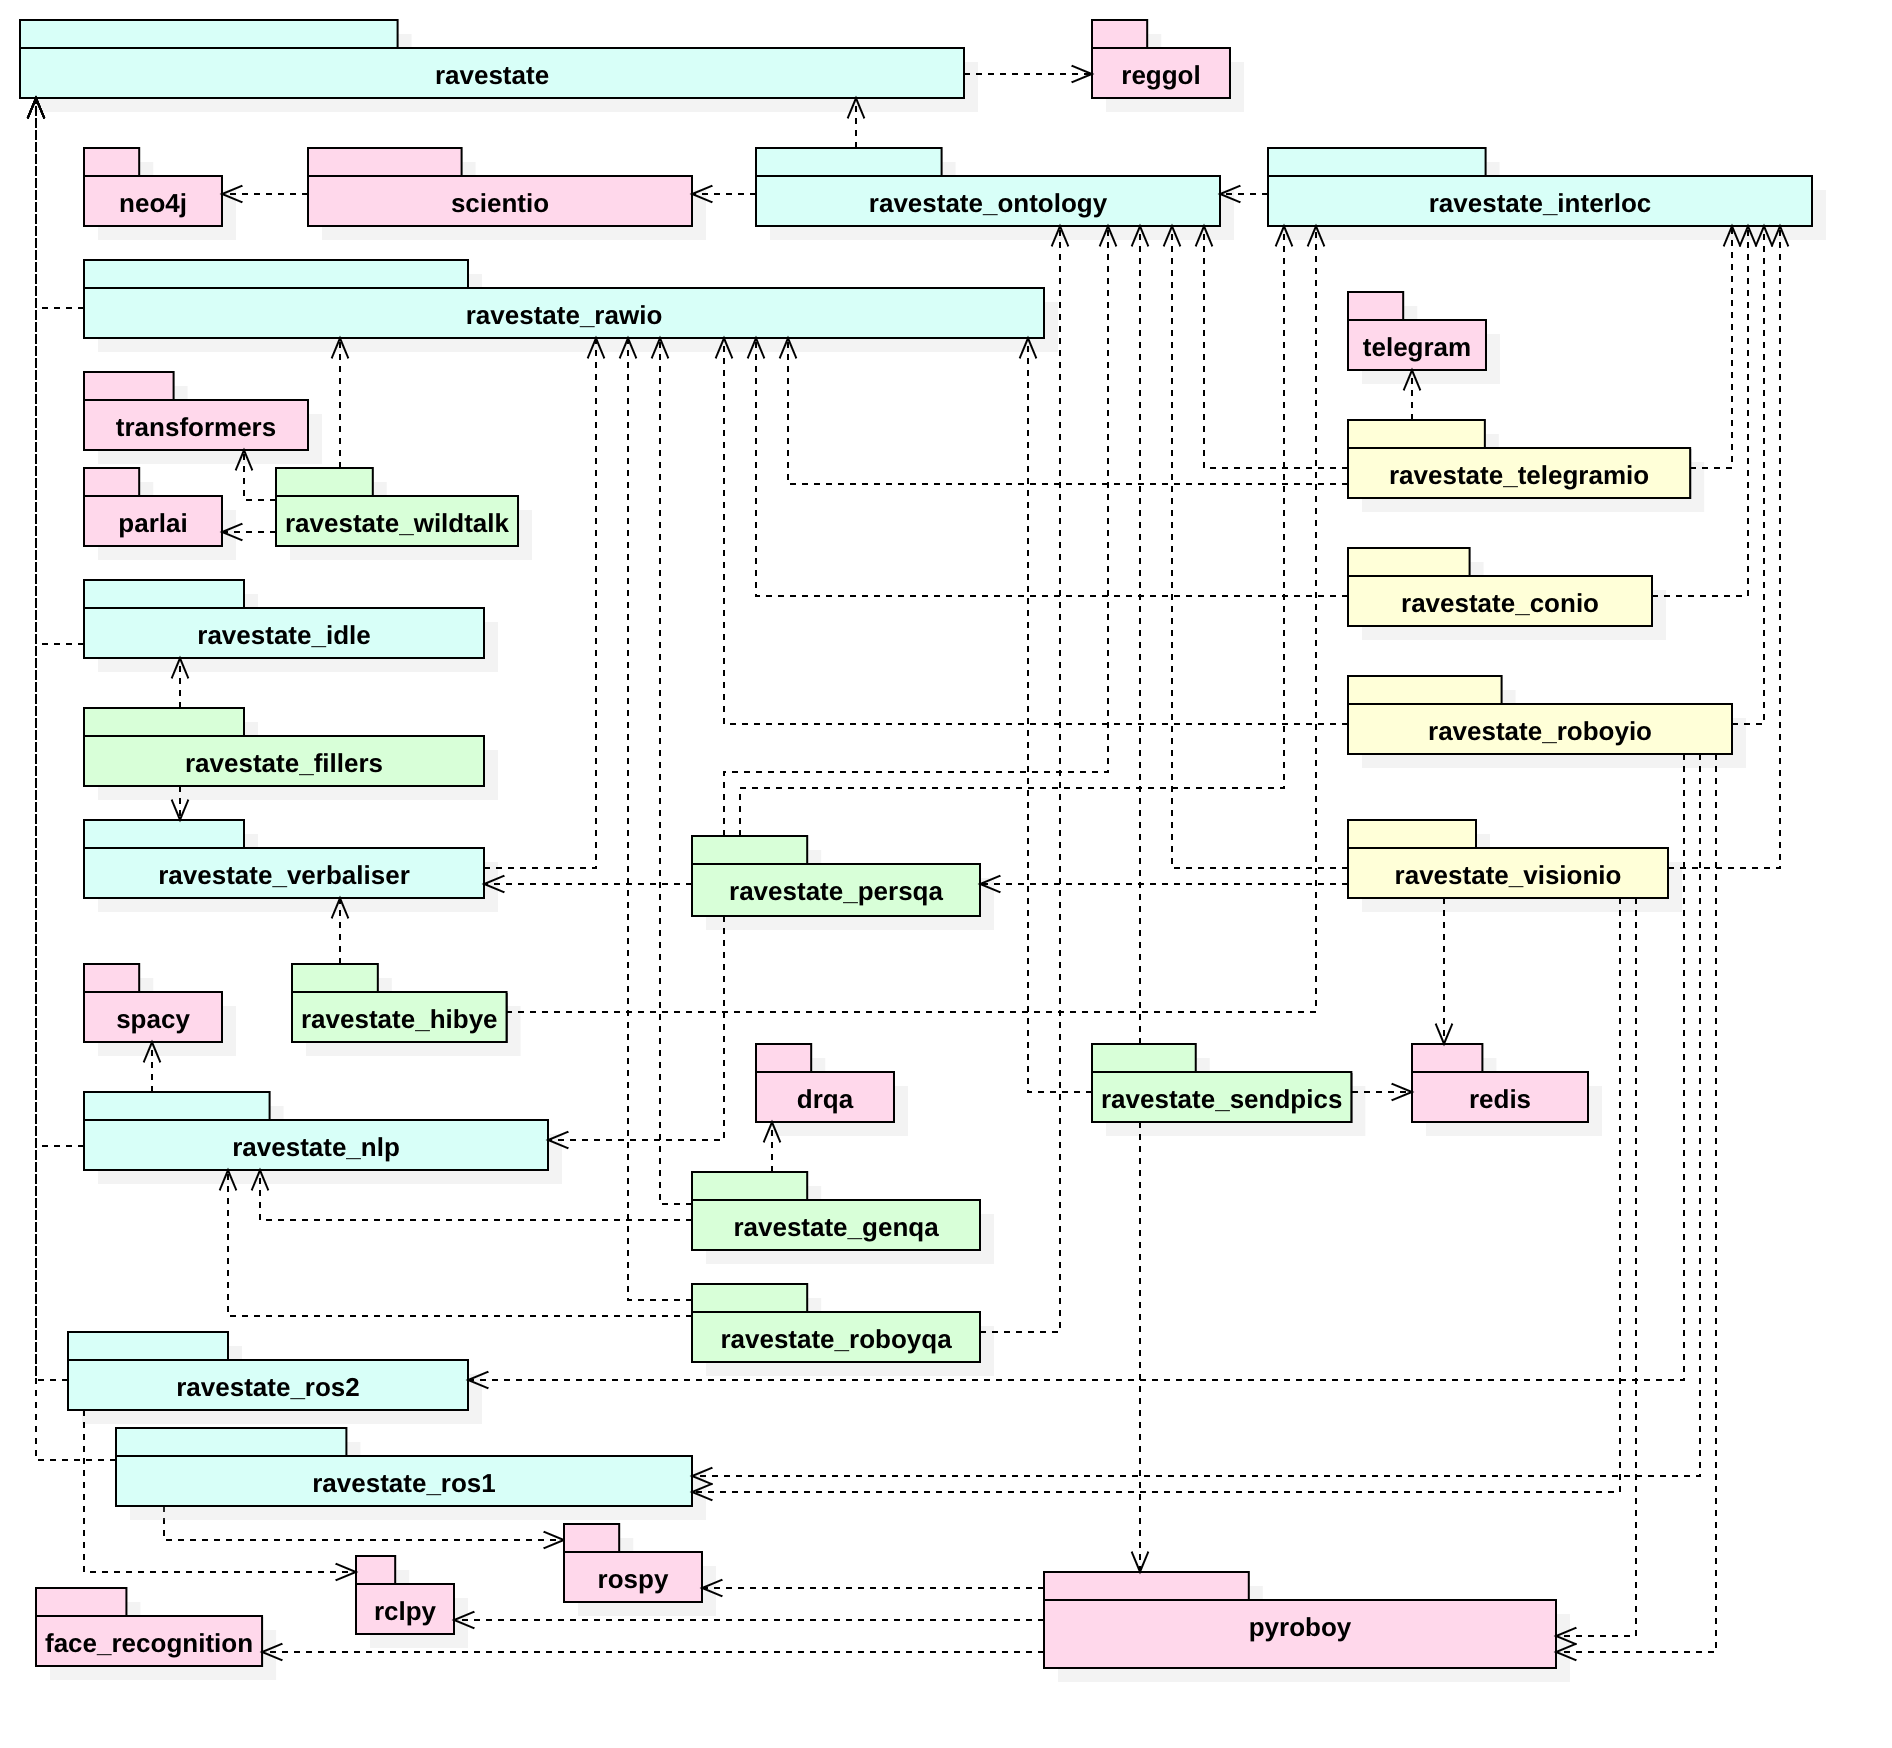
\includegraphics[width=0.8\textwidth]{figures/ravestate.png}
  \caption{The dependency diagram of Ravestate ~\parencite{ravestate}. } \label{fig:ravestate}
\end{figure}

\section{Computational Humour}

Humour is essential in interpersonal communication. It influences conversations drastically. Therefore, Computational Humour is considered an essential branch of Natural Language Processing and Computational Intelligence. Some publications report that including humour into embodied robots functionality improves HRI and makes it more pleasant for human users~\parencite{cb48d59358674187a9fccbc31a3bbd51}. 

There has been ongoing research on humour applications in the Natural Language Generation tasks such as generating canned jokes. For example, punning riddles generation:
\begin{itemize}
    \item What do you call a quirky quantifier? An odd number.
\end{itemize}
which was carried out as a symbolic description of humorous riddles and resulted in a "JAPE" project in 1994~\parencite{binsted1994symbolic}.

Another well-known experiment is the "STANDUP" - a rule-based humour production system for stand-up comedy or a more modern alternative for "JAPE", developed in 2007. It used WordNet and was capable of generating such samples as:
\begin{itemize}
    \item What do you call a cry that has pixels? A computer scream.
\end{itemize}
This experiment was the first attempt to create a joke generation system widely available to the end users~\parencite{3ae3f943de704b378c6f53fd1f0d358a}.

However, even though implementing humour processing pipelines in Dialogue Systems is advantageous not only for joke generation on the go but also for other NLG problems, there was no significant breakthrough so far. Firstly, from the Natural Language Processing perspective, the intricate semantics of humour demands a lot of creativity and deep understanding of the context which may require the human mind to produce a joke.  Secondly, humour is a multimodal interaction including but not limited to joke delivery, gestures, voice tonality, facial expressions.  

Adapting to the current context might be a critical task and research problem for Social Robots. The NLG capabilities are one of the essential functions to interact with people and other Social Robots, which means that the robot has to produce response utterances online without preparing them beforehand. Besides language processing at runtime, the robot has to evaluate the non-verbal behaviour of its conversation partners to pick up subtle cues about the current context. All of the functionality mentioned above is also necessary for humour generation tasks. 

Therefore, there are two important considerations to address:
\begin{itemize}
    \item Lack of flexibility – we would like to be able to generate a wide range of different jokes using unsupervised approaches to create a \acrlong{nlg} system. 
    \item Lack of feedback – we may never be sure if a generated joke is funny to a particular interlocutor. Thus, we need some approach to establish feedback for each conversation partner. 
\end{itemize}

Regarding the feedback problem, there is a proposed approach from researchers at the University of Augsburg. Their idea is to combine the \acrshort{nlg} and \acrfull{rl} so that a robot can adapt to the particular user’s behaviour using external signals. To develop such capability, they propose to use multimodal Human-Robot Interaction in the context of dynamic joke generation as a way of learning how to improve the robot’s perceived social intelligence. The modalities of interest are speech and video data to extract emotion-related patterns such as smiling or laughing. These modalities estimations are combined with the \acrshort{rl} mechanism to generate rewards when the estimates are positive and punish the behaviour otherwise. This approach allows to automatically adjust the \acrshort{nlg} parameter according to modality signals from the user~\parencite{ritschel-andre-2018-shaping}~\parencite{10.1145/3242969.3242976}. Figure \ref{fig:humour} illustrates the concept of the proposed approach.

\begin{figure}[htpb]
  \centering
  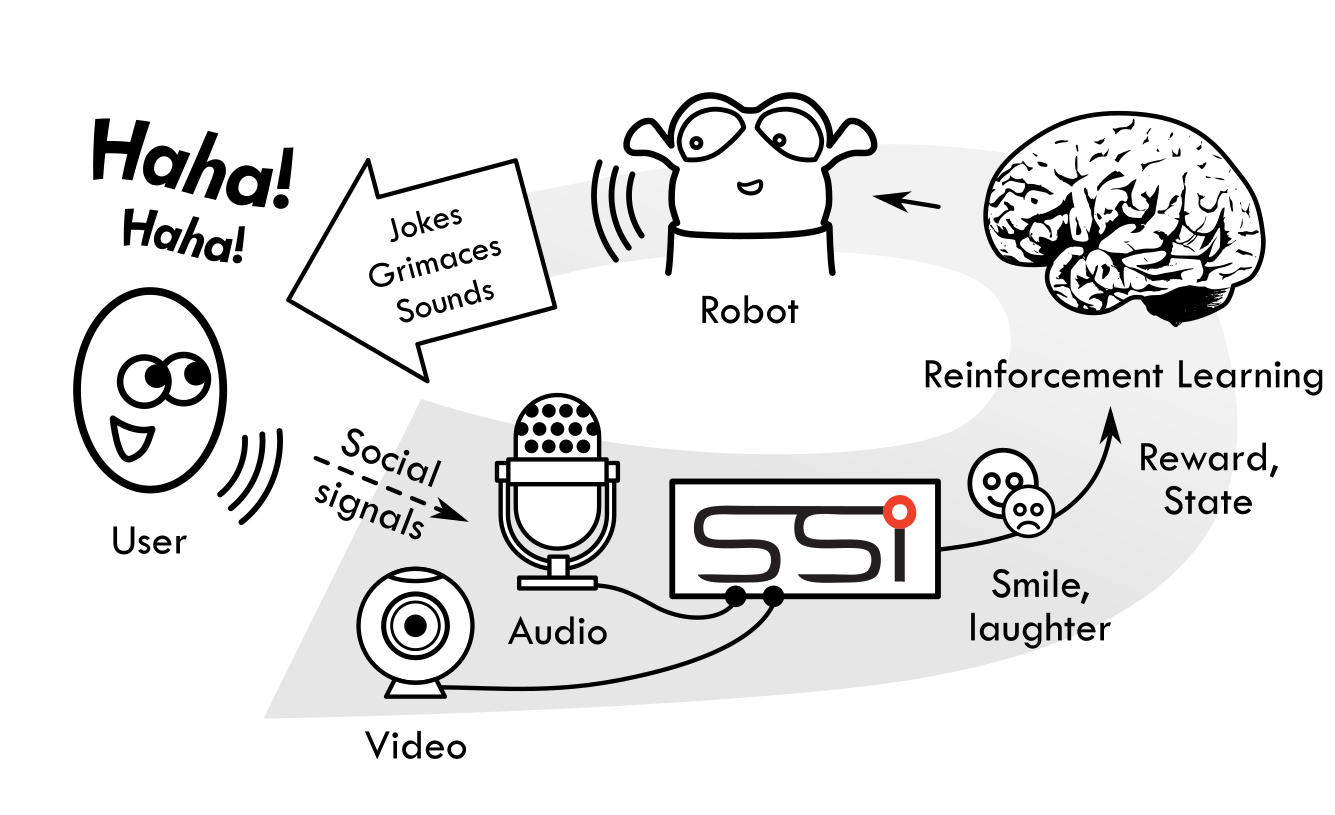
\includegraphics[width=0.8\textwidth]{figures/humour.png}
  \caption{Scenario of a robot learning to be funny from human social signals ~\parencite{10.1145/3242969.3242976}. } \label{fig:humour}
\end{figure}

Following this approach, we would also like to take image and audio data into account in our system, considering that Roboy has all of the necessary hardware for this. However, we still need a Language Model for the \acrshort{nlg} task. 

\section{Language Model}
To successfully conduct the \acrshort{nlg} tasks, we require a system that knows a probability distribution over words. Such systems are called Language Models. Natural Language Processing systems use these models to determine the necessary context to differentiate between words. Thus, given the particular word, we can predict the most probable words that could follow the initial one in the generated sentence. This capability is indispensable for humour generation tasks. Since recently, state-of-the-art Language Models have utilised Neural Networks for better performance. One of the latest such models is GPT-2 by OpenAI.

\subsection{GPT-2}

\begin{figure}[htpb]
  \centering
  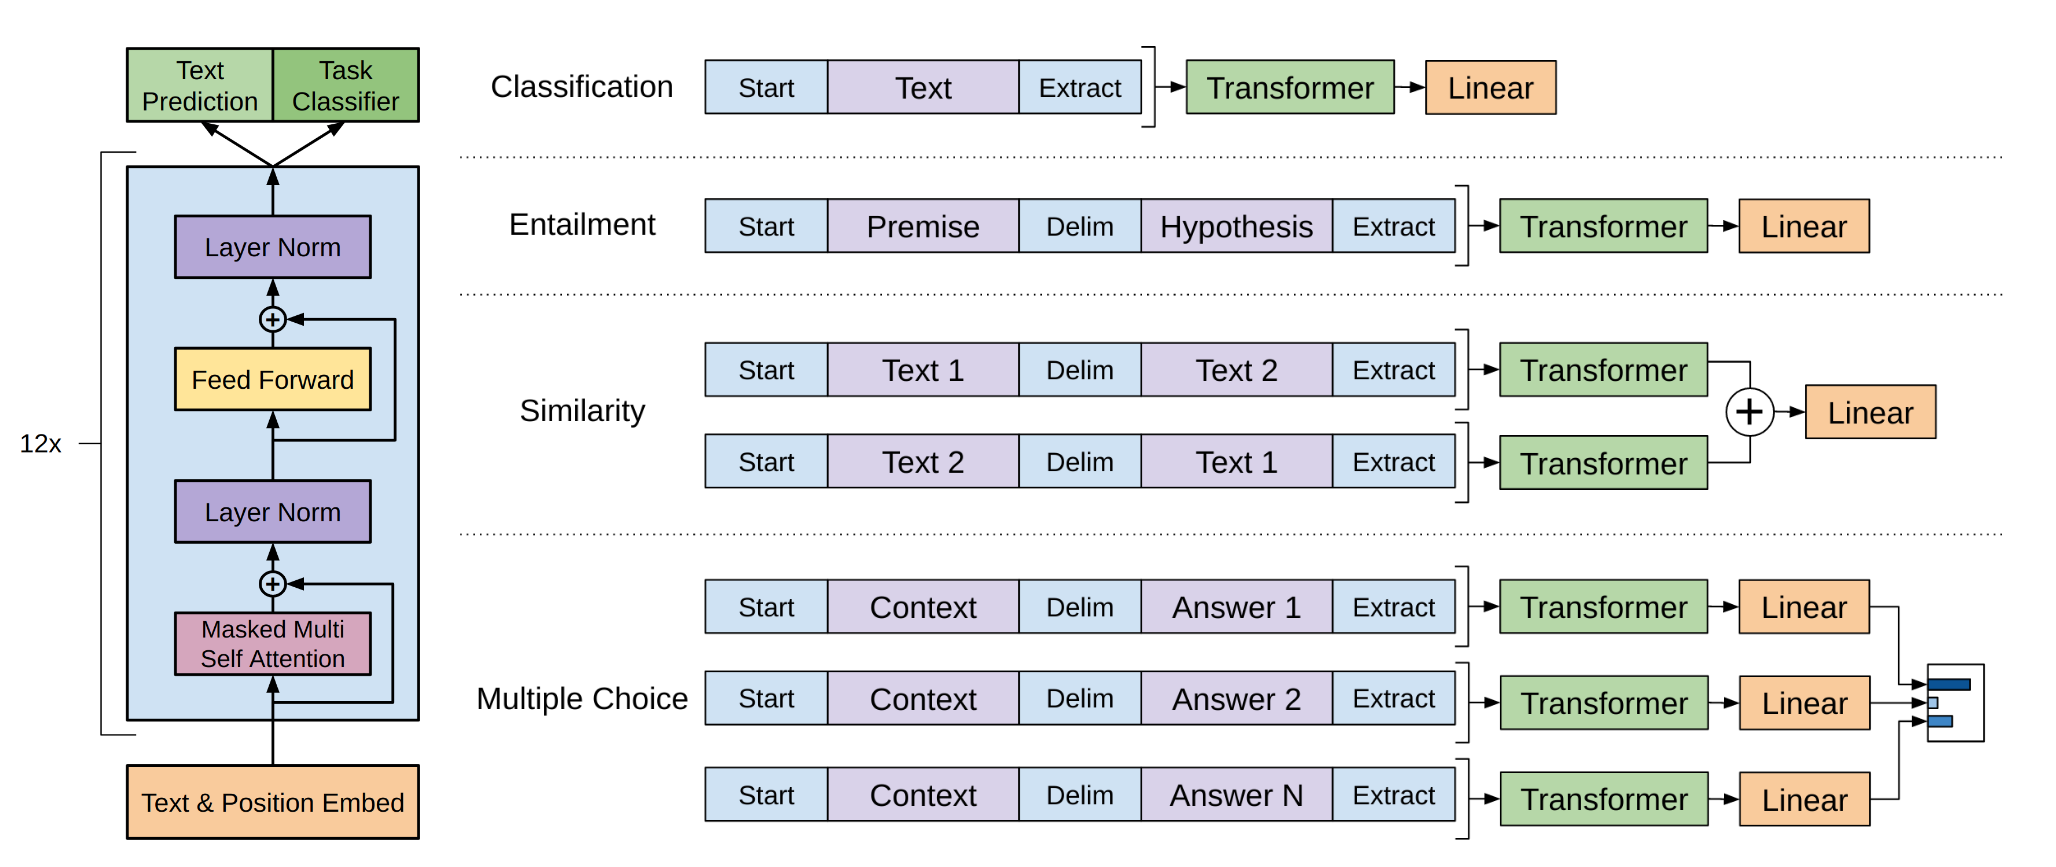
\includegraphics[width=1.0\textwidth]{figures/gpt.png}
  \caption{GPT-2 Transformer architecture and training objectives~\parencite{Radford2018ImprovingLU}.} \label{fig:gpt}
\end{figure}

OpenAI developed a new GPT-2 Language Model in 2019 based on the previous GPT model, with over 10-fold increase in parameters and used data. It employs a \acrlong{dnn} architecture to predict the next word (token) given the previous ones in the input text. The cornerstone of the architecture is the Transformer-layer (see Figure~\ref{fig:gpt}). Currently, the biggest available model contains 1.5-billion parameters. GPT-2 can learn Natural Languages tasks such as question answering, summarisation and comprehension within an unsupervised training approach while being superior to other Language Models (on 7 out of 8 tested datasets).

The GPT-2 prediction quality directly derives from the amount of training data. Therefore, the training process employed 40 GB of publicly available text from 8 million online sources which allow generating naturally sounding sentences due to the diversity of the dataset and the data domains. However, the creators reported that might take several prediction attempts until the model outputs a satisfactory sample given how broadly the topic was covered in the original data with up to 50\% success rate. For our \acrshort{nlg} task, humorous data naturally belongs to numerous domains. However, there are usually many samples that use similar lexical and vocabulary structure. A good example is the "chicken" riddle. Usually, it starts with: "Why did the chicken cross the road?" Then, follows the punchline – anything silly or absurd: from obvious "To get to the other side" to "She was afraid someone would Caesar!" Structurally, this type of jokes is very rigid. Therefore, we would like to see how well GPT-2 will perform on our data ~\parencite{radford2019language}.

\section{Automatic Emotion Recognition}

The visual and audial cues can be crucial for humorous HRI applications similarly to how human psychology shapes the perception of verbal interaction. Given visual or auditory stimuli, humans often gauge the seriousness of the situation based on facial expressions as well as timbre\footnote{the character or quality of a musical sound or voice as distinct from its pitch and intensity} and cadence\footnote{a modulation or inflexion of the voice} in social interaction. Therefore, we need a feedback mechanism to evaluate users' emotions. 

To help Roboy to recognise and evaluate emotions of conversation partners, we have decided to adopt two following technologies to use in our implementation. The first one is the EmoPy package that offers facial emotion recognition using a frame-by-frame video stream. Another one is \acrfull{ser} - it provides emotion recognition result based on audio recordings. \acrshort{ser} is a part of the bigger Multimodal Emotion Recognition project~\parencite{maelmer}.

\subsection{EmoPy}

Developed at ThoughtWorks Arts, EmoPy is a Facial Expression Recognition (FER) package. The package offers various Neural Network architectures trained on facial expression data. The available pre-trained models use the Microsoft’s FER+ dataset because it is the best currently available open-source dataset for FER~\parencite{emopy}.

FER+ is a dataset based on the previous Microsoft FER data. With the help of ten crowd-sourced taggers, creators of the dataset re-labelled all data points to improve the ground truth quality on each image. Similarly to original FER, FER+ offers still-image emotion data and labelling \parencite{BarsoumICMI2016}.

Using FER+ labels, EmoPy can recognise seven available emotions such as calm, anger, disgust, fear, happiness, sadness, and surprise. The best available EmoPy model uses a Convolutional Neural Networks (CNN) architecture (see Figure \ref{fig:emopy}). The software implements the Neural Network modules via the Keras framework employing Tensorflow as the backend~\parencite{emopygh}.

EmoPy is an open-source project available through PyPi package management system and as source code on GitHub~\parencite{emopygh}.

\begin{figure}[htpb]
  \centering
  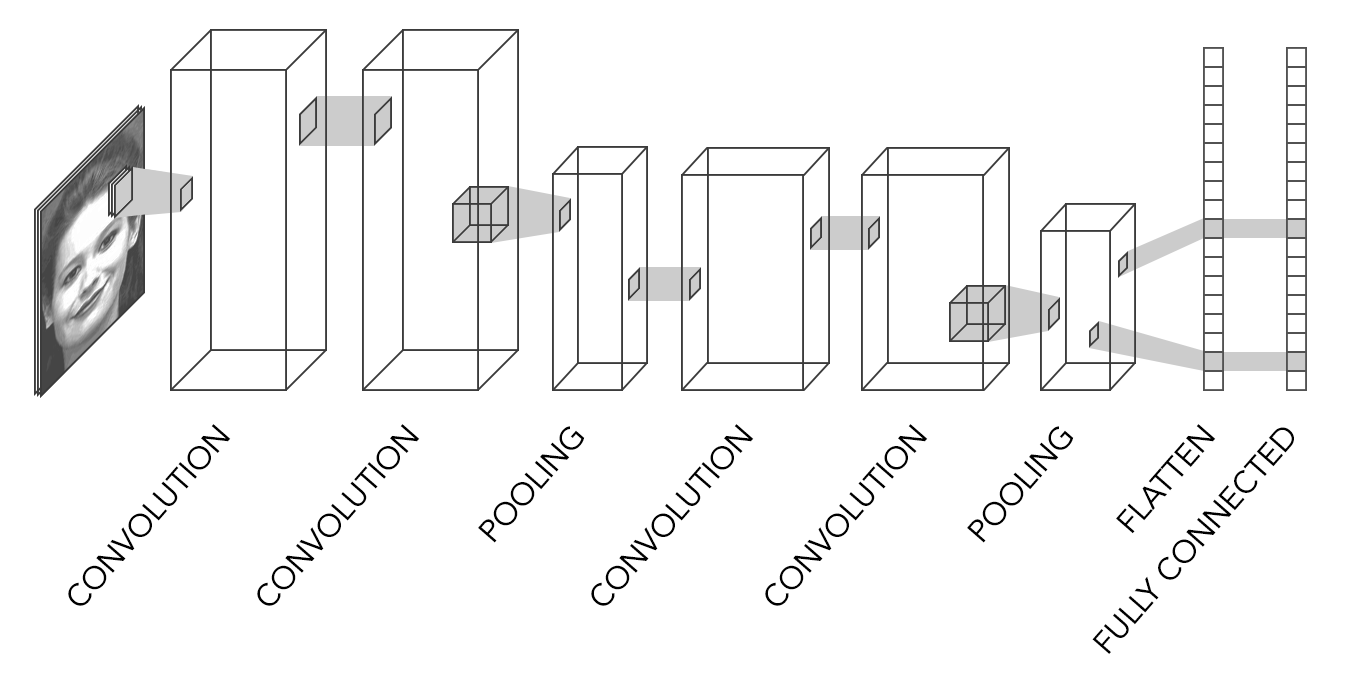
\includegraphics[width=0.8\textwidth]{figures/emopy.png}
  \caption{EmoPy CNN architecture~\parencite{emopygh}.} \label{fig:emopy}
\end{figure}

\subsection{Speech Emotion Recognition}

The \acrlong{ser} is a technology that analyses emotions expressed in speech patterns given a wave recording of the person speaking. We used the \acrshort{ser} package from the Multimodal Emotion Recognition project. The \acrshort{ser} package employs Machine Learning models trained on the Ryerson Audio-Visual Database of Emotional Speech and Song (RAVDESS) dataset. 

The dataset comprises 7356 data points. To create each sample, 24 (12 female, 12 male) professional voice actors participated in recording spoken utterances in a neutral North American accent. Each file consists of two matching utterances. The samples were recorded at two levels of emotional intensity, either normal or strong. The emotion labels comprise calm, happy, sad, angry, fearful, surprise, and disgust. To assign labels to each of the samples, 247 untrained researchers from North America provided ten ratings for each file with regard to its validity, intensity, and authenticity~\parencite{livingstone_steven_r_2018_1188976}.

The Multimodal Emotion Recognition project is open-source software distributed under Apache License 2.0 and developed for the French employment agency Pole Emploi. The goal is to create a platform for job-seekers which will help the candidates by analysing their verbal and non-verbal behaviour. The \acrshort{ser} offers Support Vector Machine and Time Distributed Convolutional Neural Network models. Given the higher accuracy provided by the CNN model, we will use it in our implementation. Figure \ref{fig:ser} illustrates the architecture of the model. 

\begin{figure}[htpb]
  \centering
  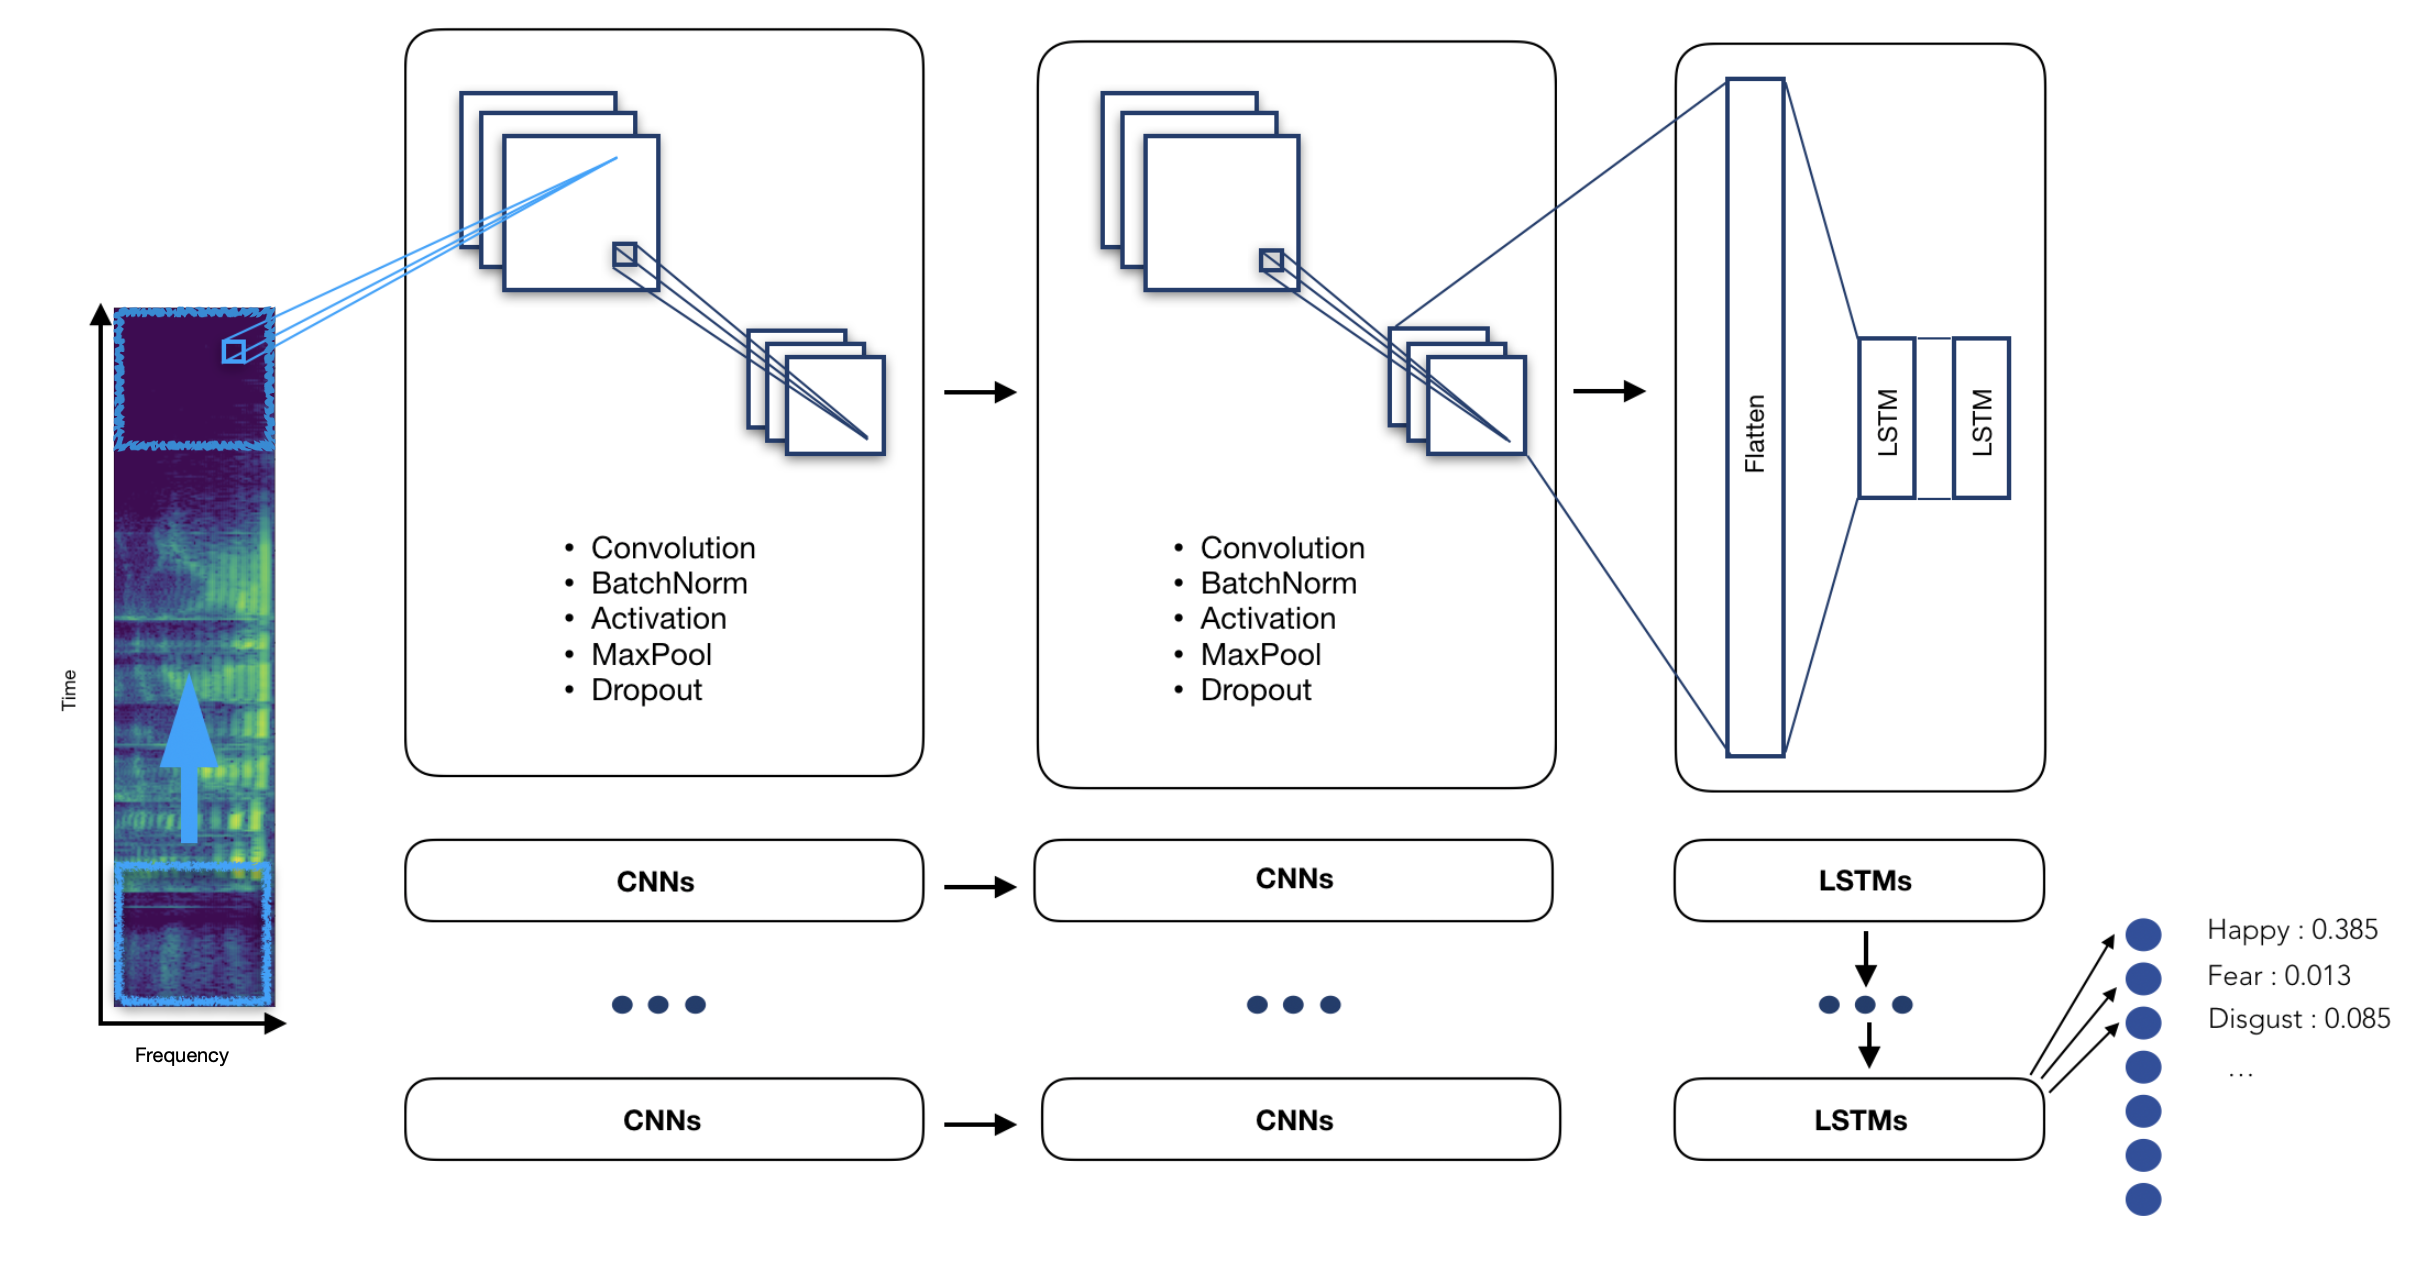
\includegraphics[width=1.0\textwidth]{figures/ser.png}
  \caption{\acrshort{ser} Time Distributed CNN architecture. [github]} \label{fig:ser}
\end{figure}

The idea behind the architecture it to employ a rolling window technique along the mel-spectrogram. Afterwards, each of the resulting window output constitutes an input to the Convolutional Neural Network layers. These layers consist of four Local Feature Learning Blocks (LFLBs). Then, the values are fed into the next neural network comprising 2-cells LSTM (Long Short Term Memory) model. At the end of the model pipeline, there is a softmax-activated Fully Connected (FC) layer which outputs the emotion labels for the speech samples ~\parencite{maelmer}.